\section{Results}
\label{sec:results_ukb_assoc}

\subsection{Descriptive Statistics}
\label{sub:descriptive_statistics}

Sex and age of participants is affecting both main and secondary phenotypes (see Figure~\ref{fig:disc}).
One can observe noticeable sex differnces in risk taking, alcohol consumption as well as neuroticism.
As expected, risk taking is more prevalent in male than in female subjects. 
Similar, man seem to drink more alcohol than women.
The opposite seems to be the case for neuroticism.
Women have, on average, higher neuroticism scores than man.
Further,  while sex differnces are minor within impulsive aggression it is interesting that more women compared to man seem to expres impulsive aggressive behaviors, thus contrasting earlier results in Chapter~\ref{chap:long_hera}. 

Similar to the effect of sex, age seem to have some influence on aggression, risk taking and neuroticism, but only to a lesser extend to smoking and alcohol intake.
Risk taking, neuroticism and impulsive aggression seem to decline by age, while alcohol consumption seems rather stable.
Further, one can observe that older individuals are more likley to currently smoke, or have smoked in the past.
A result which is not particular surprising.
Furthermore, these result suggest that a genome wide association study should include both age and sex as covariats.

\begin{figure}[htpb]
  \centering
  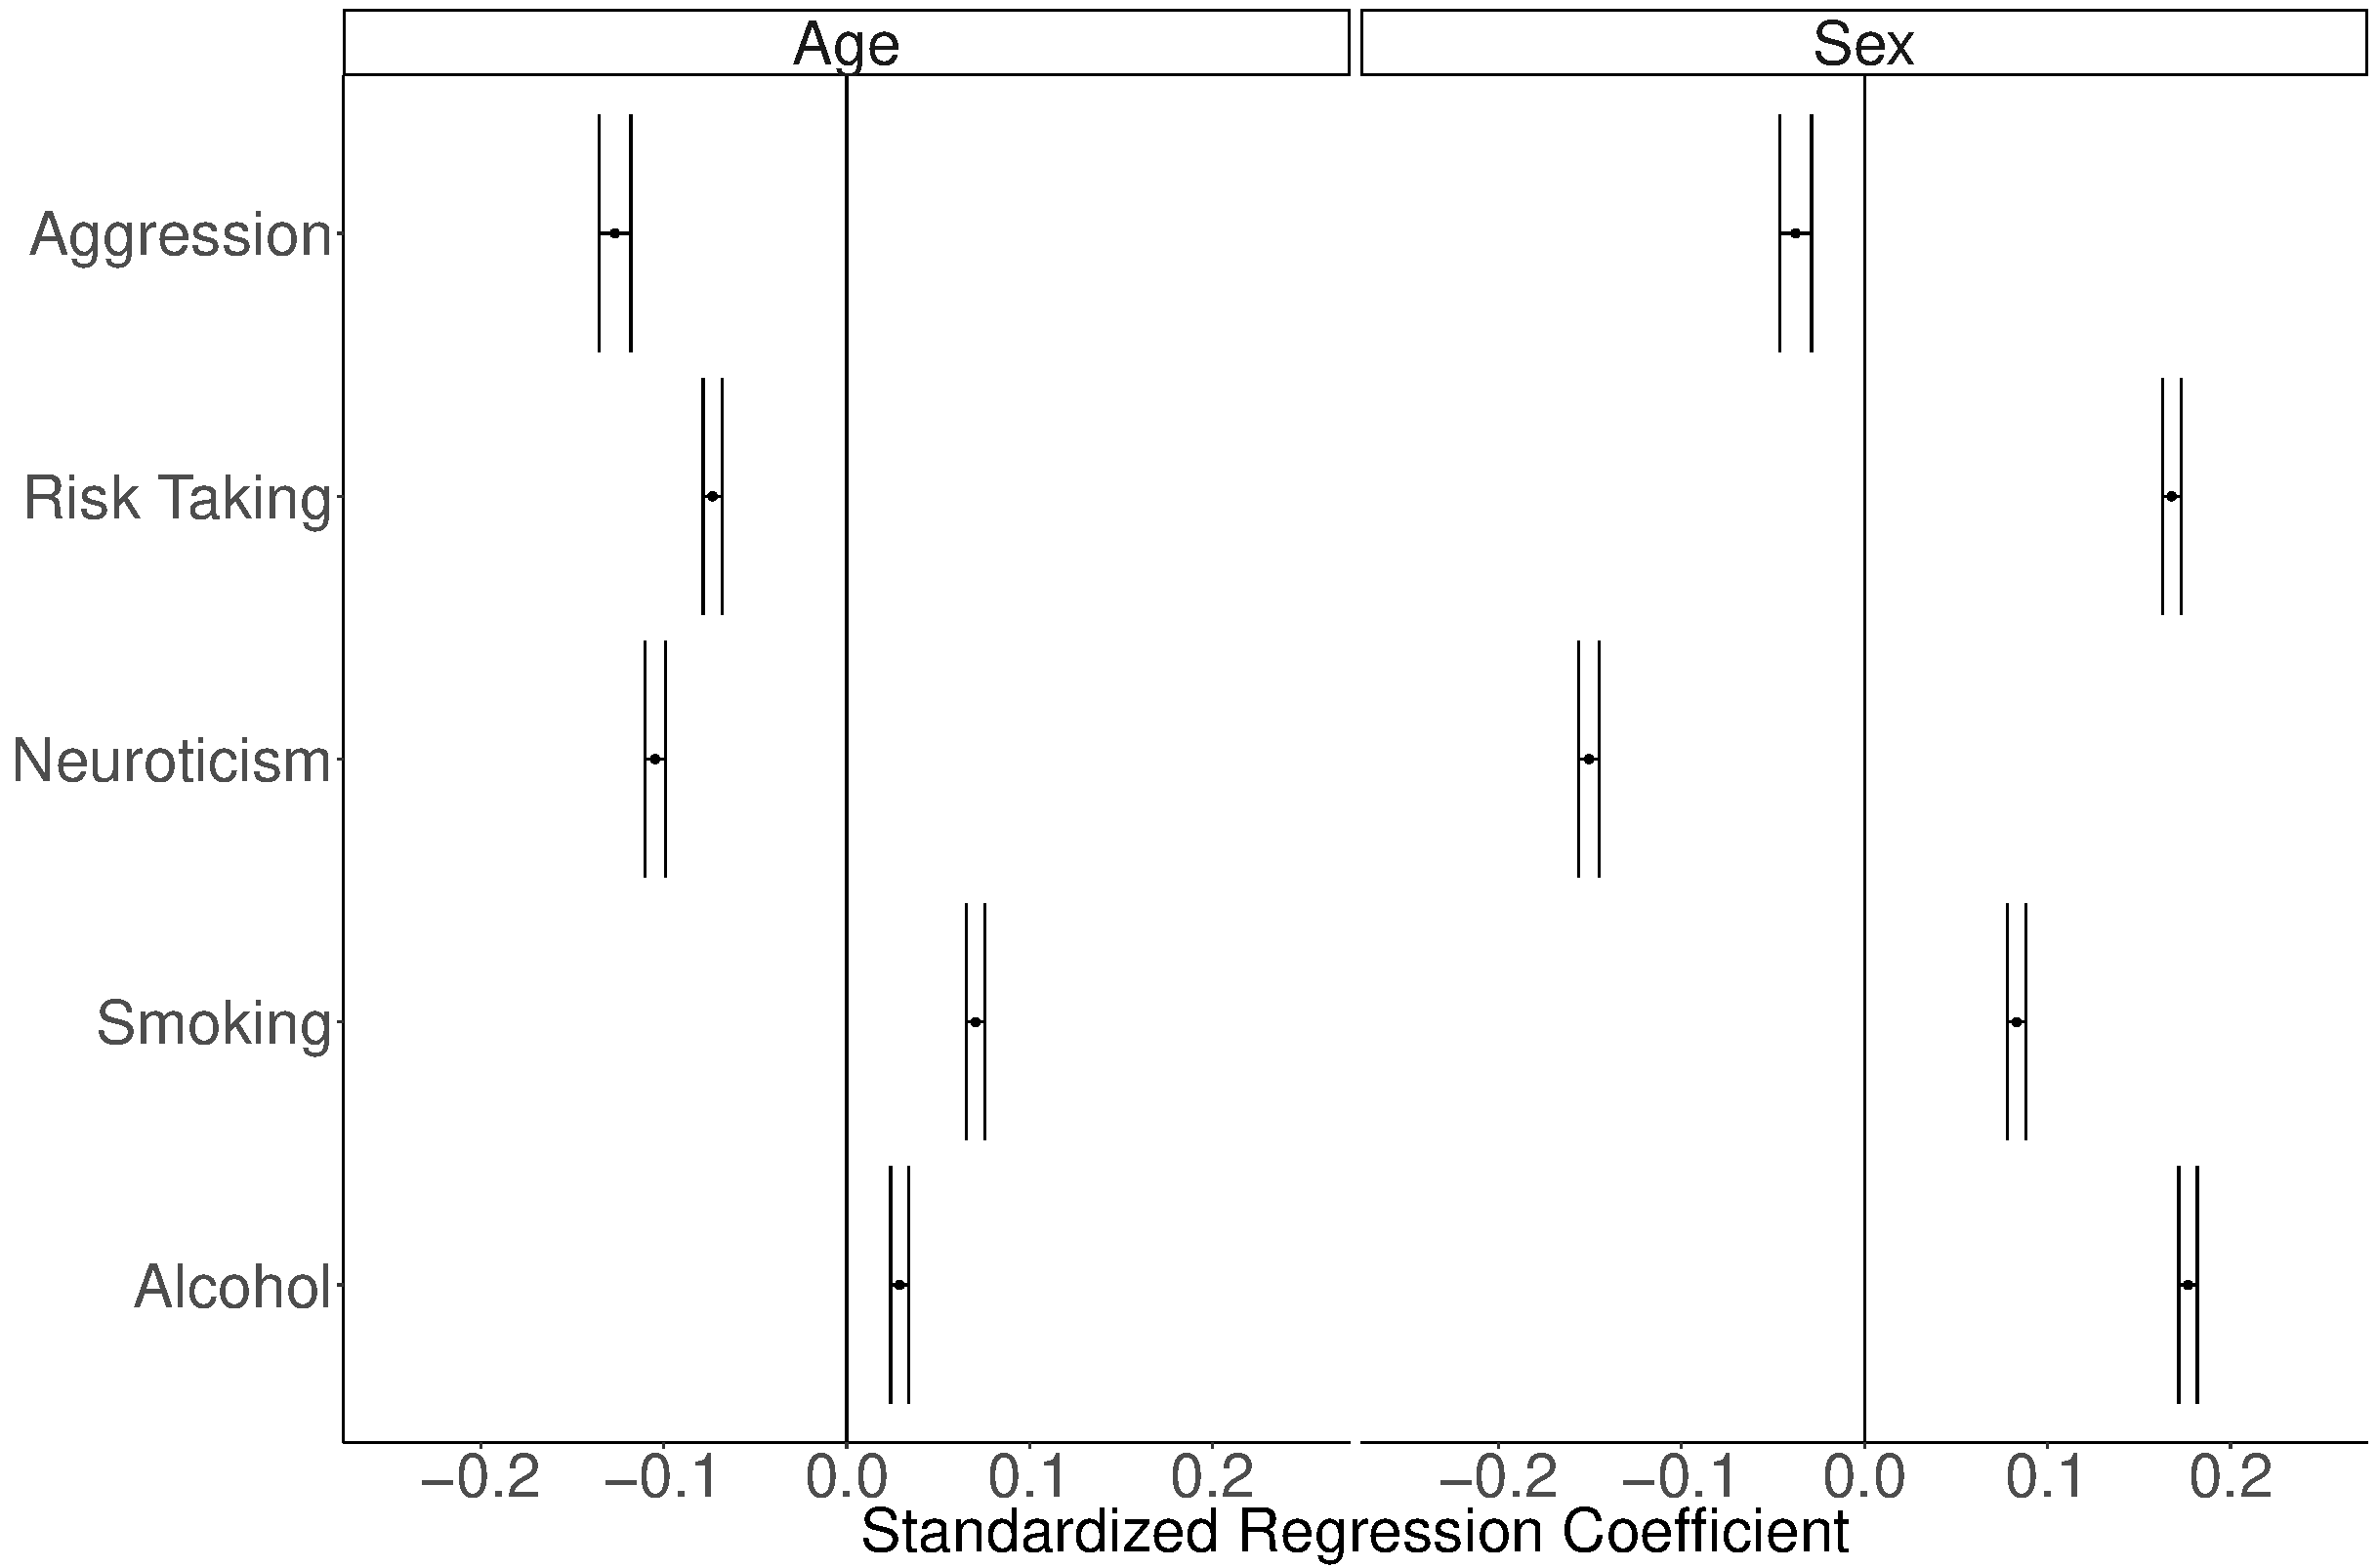
\includegraphics[width=0.8\linewidth]{ukb_assoc/figure/phenotype/descriptives_plots.pdf}
  \caption{
    Descriptive Statistics of primary and secondary phenotypes for all participants.
    (A) Standarized effect of sex (male, female) on phenotypes. 
    A possitive effect size indicates creater prevalance in male than in female.
    Errorbars indicate the 95\% confidence interval.
    (B) Standarized effect of age on phenotypes.
    Errorbars indicate the 95\% confidence interval.
    (C) Barplot of neuroticism.
    The plot displays the frequency of each neuroticism score.
    (D) Barplot of alcohol intake.
    The plot displays the frequency of each alcohol intake score.
  }\label{fig:disc}
\end{figure}

\subsection{Phenotype Correlations}
\label{sub:phenotype_correlations}

Phenotypical correlations are displayed in Figure~\ref{fig:corr_pheno}. 
All correlations were significant at $p\leq 0.05$ after adjusting for multiple testing using the Bonferroni correction.
Correlations between risk taking and impulsive aggression is with $r(48,540)=0.09 (p\leq0.0025)$ relatively small
and I was unable to detect larger effects between impulsive aggression and alcohol consumption ($r(50,220)=-0.05, p\leq0.0025$)
as well as smoking ($r(50,106)=0.1, p\leq0.0025$).
Similar, risk taking displays only small correlations between
smoking ($r(146,051)=0.00, p\leq0.0025$),
alcohol consumption ($r(146,350)=0.06, p\leq0.0025$)
and neuroticism ($r(120,201)=-0.03, p\leq0.0025$). 
Nevertheless, medium correlations were present between impulsive aggression and neuroticism ($r(41,420)=0.33, p\leq0.0025$).

\begin{figure}[htpb]
  \centering
  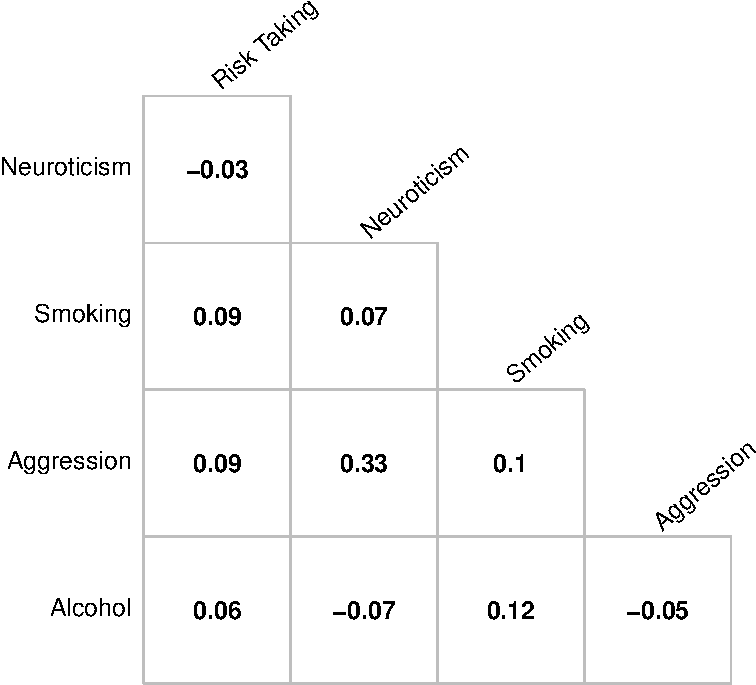
\includegraphics[width=0.6\linewidth]{ukb_assoc/figure/phenotype/corr_plot_ci.pdf} 
  \caption{
    Phenotypical correlations among analysed phenotypes for all subjects.
    Displayed correlations were all significant after adjusting for multiple testing using the Bonferroni correction.
    In contrast to the genetic correlations, Caucasian and non-Caucasian subjects were used.
  }\label{fig:corr_pheno}
\end{figure}

\subsection{GWAS on impulsive aggression and risk taking}
\label{sub:gwas}

Genome wide association analysis reveled no genome wide significant loci in $37,320$ impulsive aggression subjects.
Observed SNP heritability was estimated at $5.32\% (SE=0.012)$ and are in line with previous estimated SNPs heritabilities in behavioral traits.

The genome wide association study on risk taking yield two genome wide significant loci in $120,286$ subjects in chromosome 3 and 6.
Total observed SNP heritability is with $5.52\% (SE=0.0052)$ similar to that of impulsive aggression.
The ratio between the LD-score regression intercept $\beta_0$ and the mean of the $\chi^2$-test statistics ($(\beta_0 - 1)/(mean(\chi^2)-1)$),
which indicates the proportion of inflation to factors other than polygenic heritability, is with $0.0422$ ($SE=0.052$) neglectable.
In addition, $\beta_0$ approaches 1 ($\beta_0=1.0082, SE=0.0056$) thus suggesting no population stratification (see Figure~\ref{fig:riskqq}).

\begin{figure}[!htpb]
  \begin{subfigure}{1\textwidth}
  \centering
  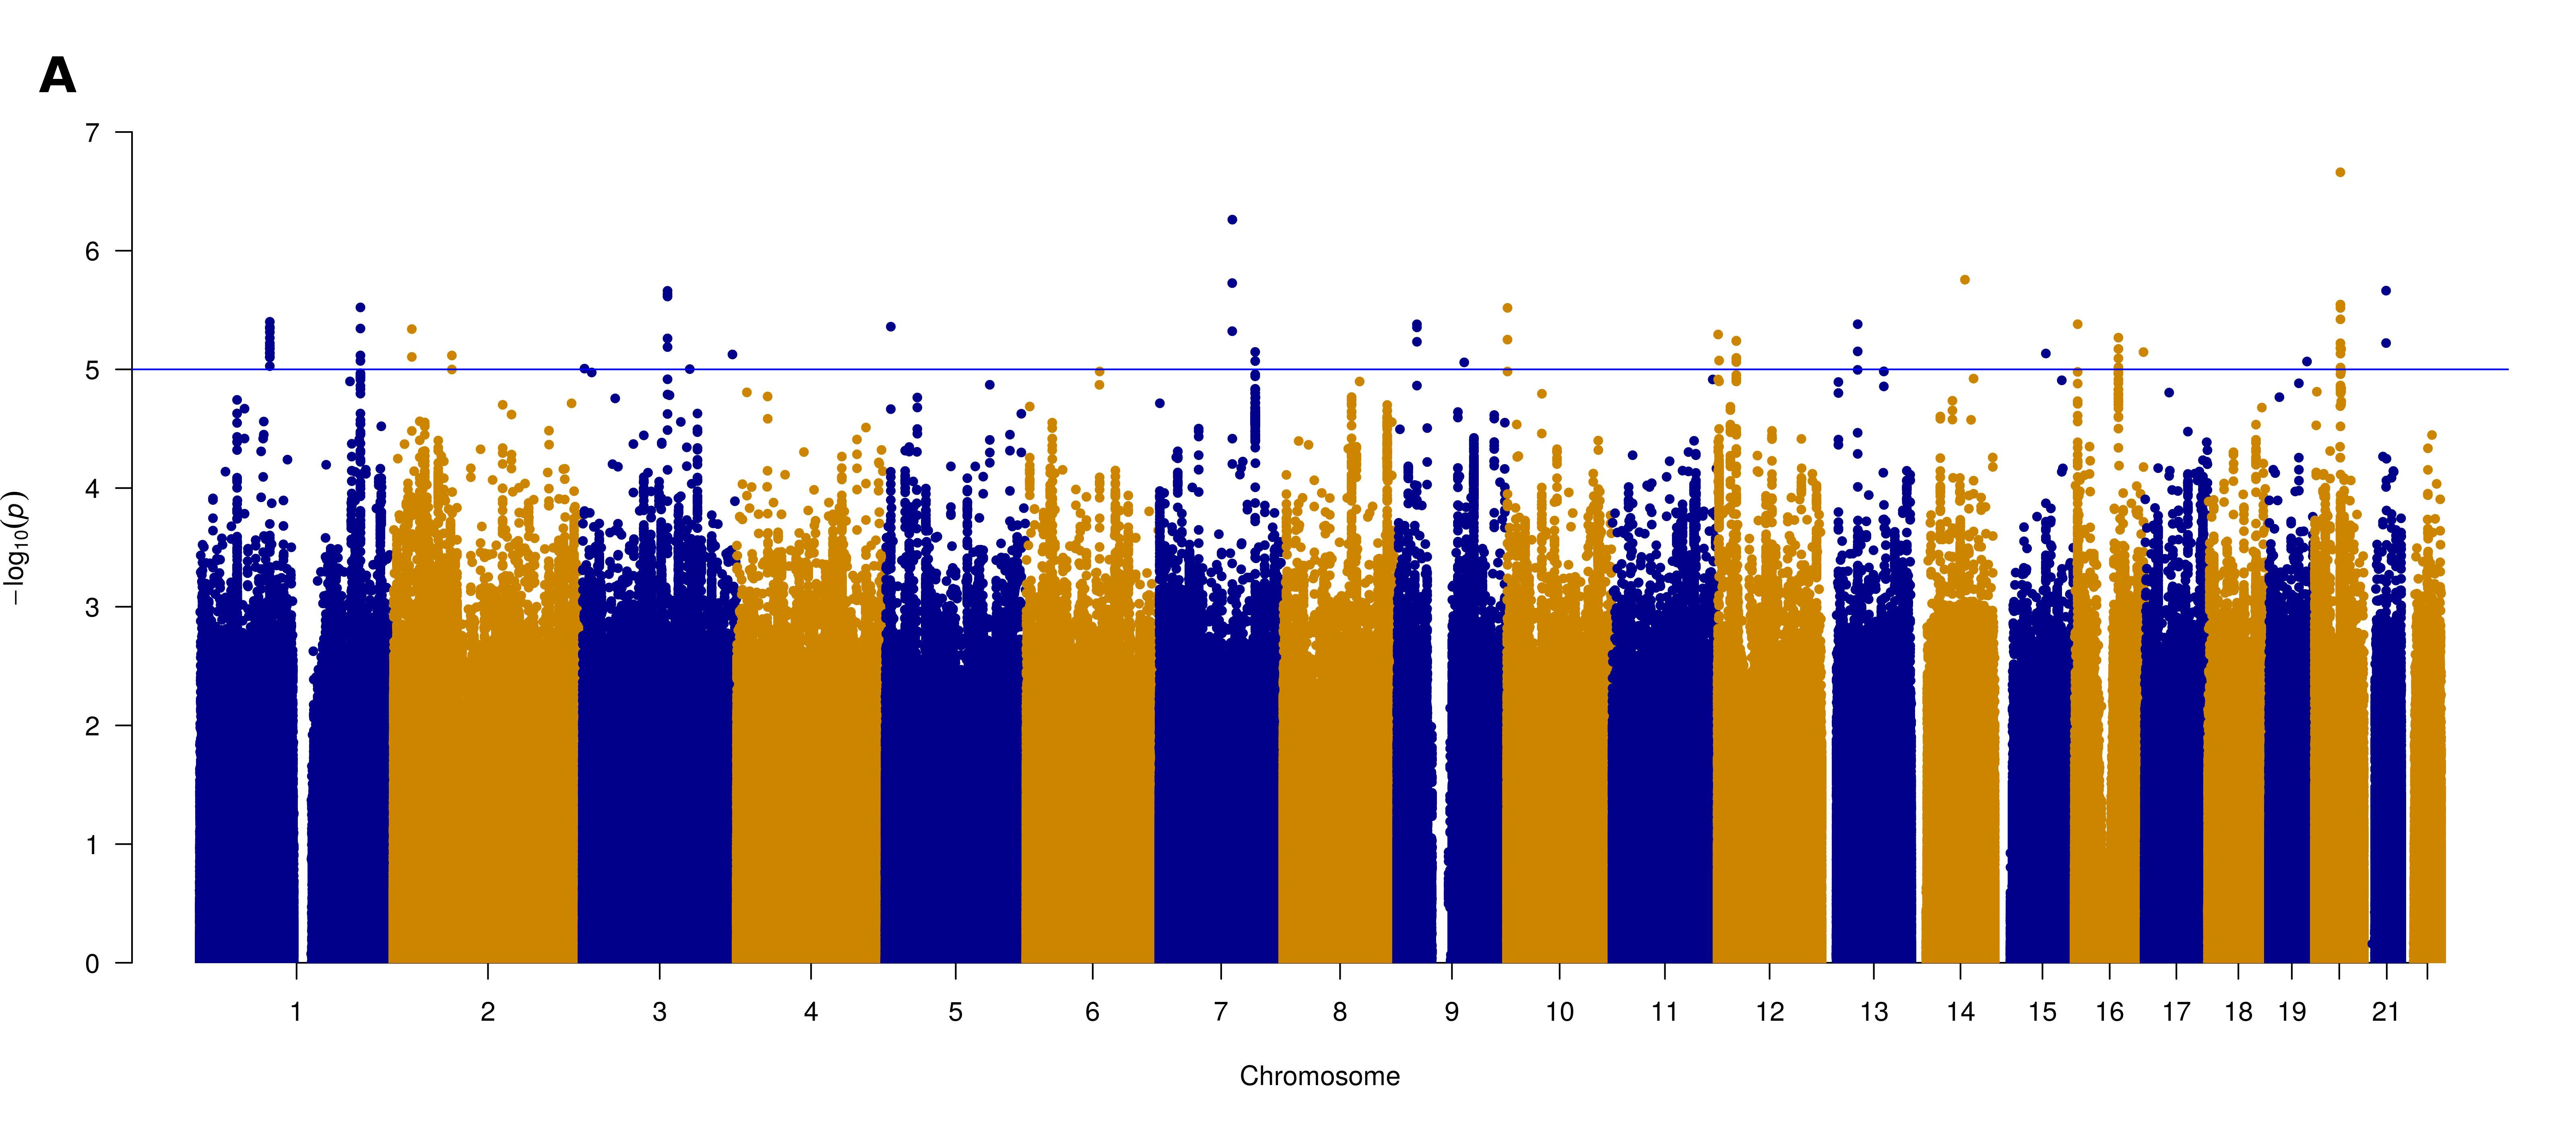
\includegraphics[width=0.8\linewidth]{ukb_assoc/figure/manhatten_plots/agg_manhatten_color_2_A.jpeg}
  \end{subfigure}
  \begin{subfigure}{1\textwidth}
  \centering
  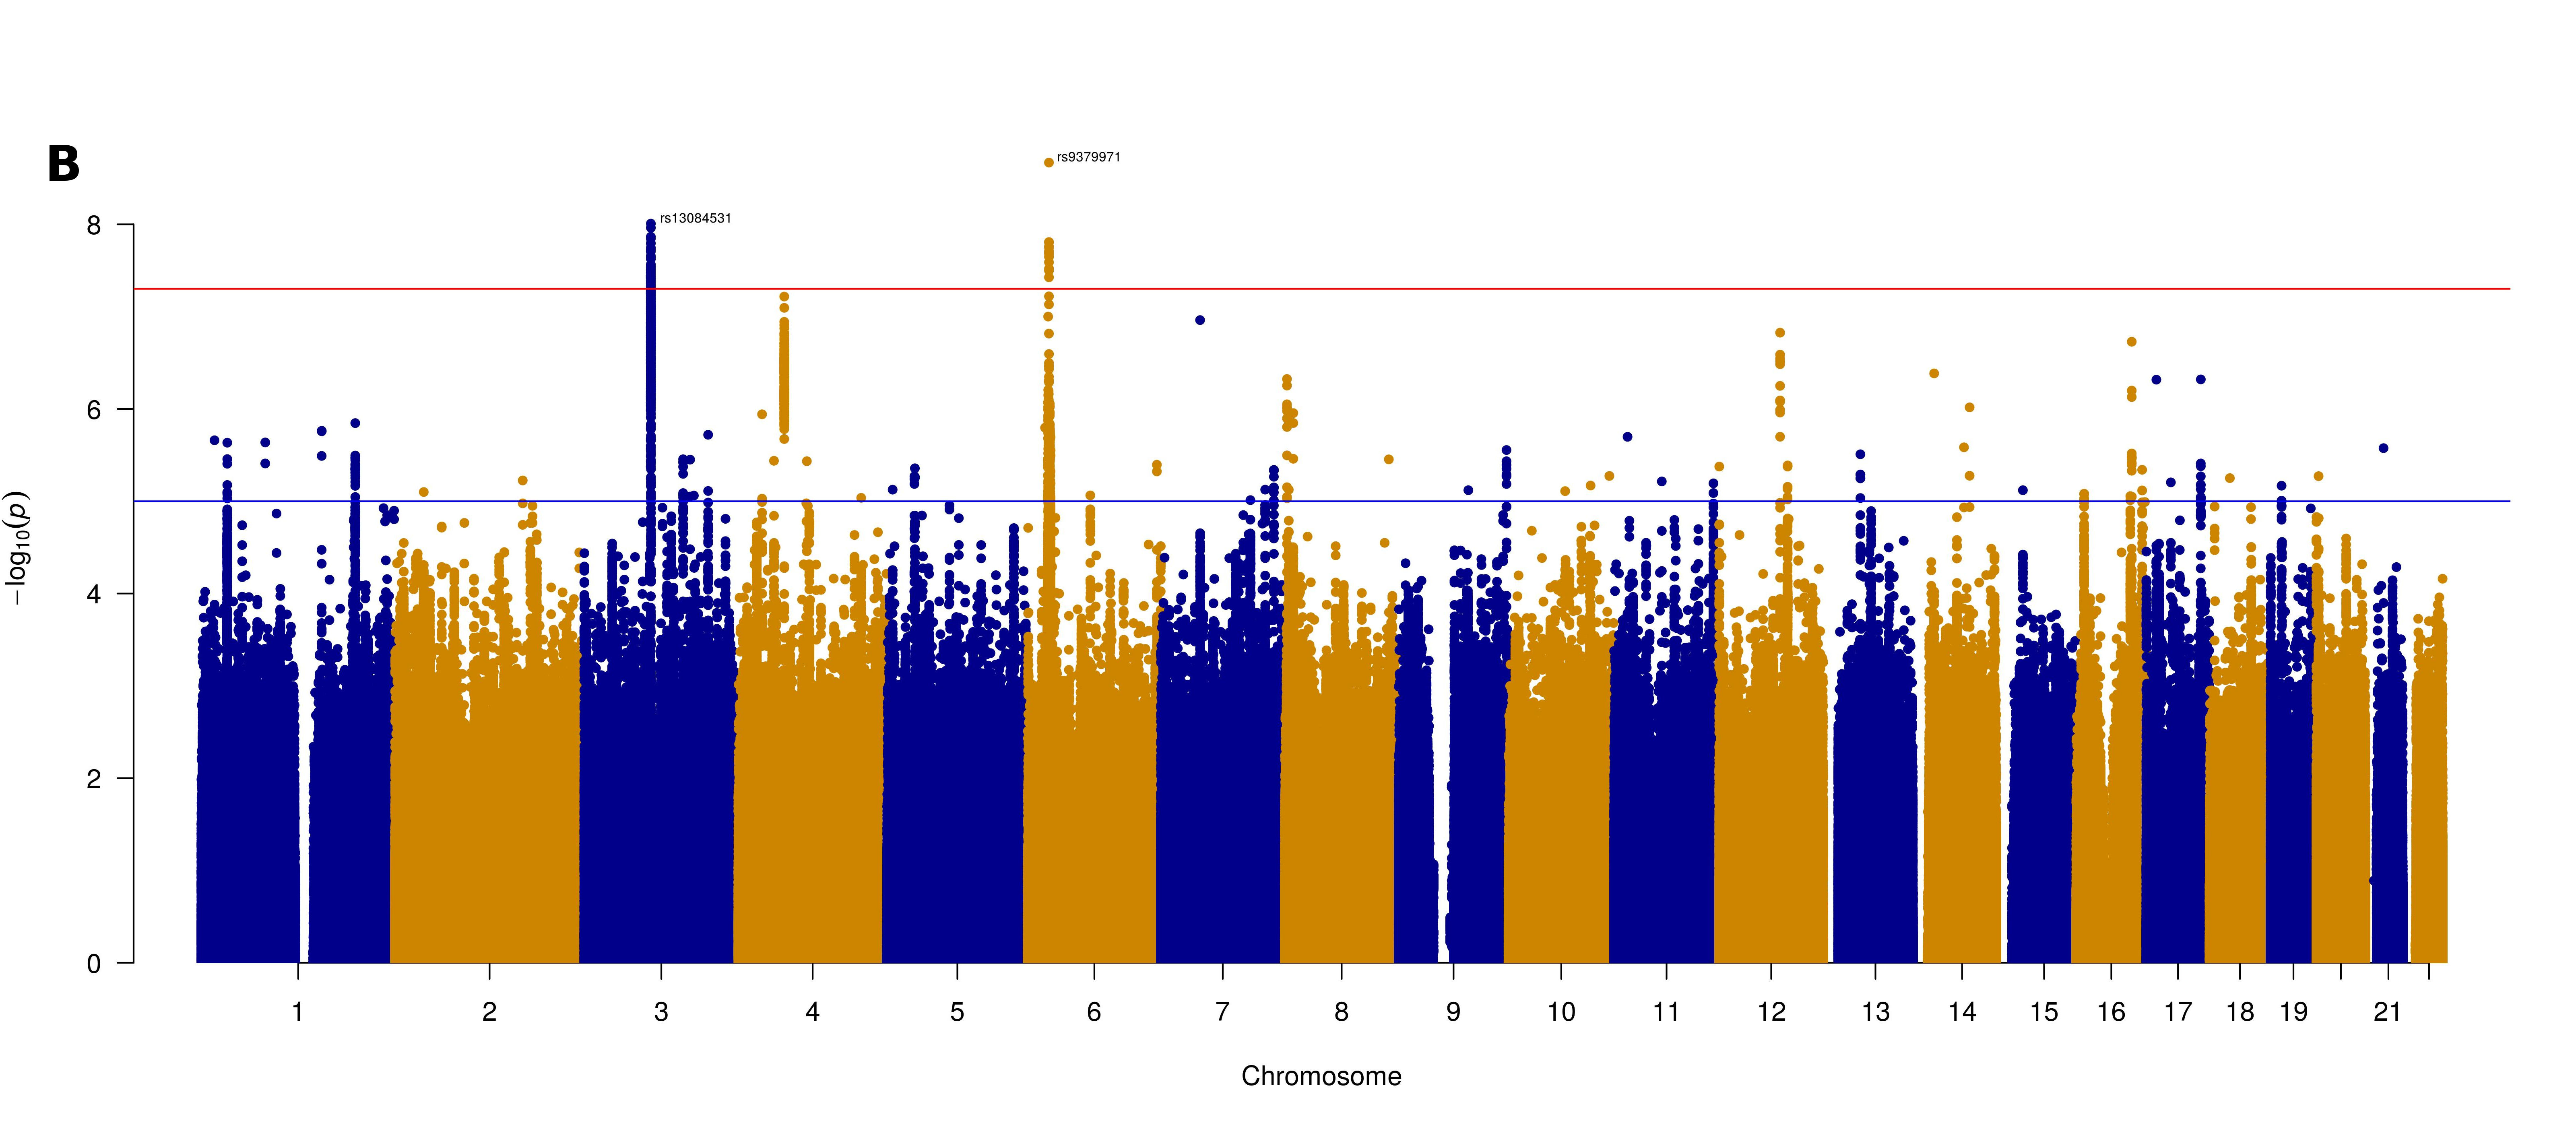
\includegraphics[width=0.8\linewidth]{ukb_assoc/figure/manhatten_plots/risk_manhatten_color_B.jpeg}
  \end{subfigure}
  \caption{
    Manhattan Plot for impulsive aggression (A) and risk taking (B).
    The red line indicates genome wide significance level at $\alpha=5\times10^{-8}$.
    The blue line represents a suggestive genetic effect at $\alpha=5\times10^{-5}$.}
\end{figure}

Closer inspection of the signal in chromosome 3 shows 2 lead SNPs namely \textit{rs1308431} and \textit{rs7639518} (see Table~\ref{tab:lead_snps_risk}).
However, \textit{rs1308431} and \textit{rs7639518} have opposite directions of effect.
The independence of these two signals was investigated using a conditional analysis.
Thus, genotypes of \textit{rs7639518} were regressed on the phenotype while adjusting for \textit{rs1308431}.
This conditional model indicates that \textit{rs7639518} is not independent of \textit{rs1308431} at a genome wide level ($OR=0.957, t(107737)=-3.787, p=0.0001523$).

\paragraph{rs9379971}
\label{par:rs9379971}
This particular variant has the strongest association among all tested SNPs with a p-value of $2.14\times10^{-9}$ (see Figure~\ref{fig:rs9379971}). 
The SNP is an intronic variant, without any mentioning in the GWAS catalog~\cite{Welter2014}.
The SNPs has been associated with \textit{POM121L2} and the region has been connected with schizophrenia across multiple studies~\cite{Aberg2013,Shi2009}.
However, the function of \textit{POM121L2} is not well understood.

\paragraph{rs13084531}
\label{par:rs13084531}
This SNP has a comparable p-value ($9.826\times10^{-9}$) and is an intron variant within the gene \textit{CADM2}.
The gene has been associated with BMI~\cite{Speliotes2010} as well as executive functions and processing speed~\cite{Ibrahim-Verbaas2015}.
Interestingly the SNP associated in the study by~\cite{Ibrahim-Verbaas2015} (\textit{rs17518584}) is in LD with \textit{rs13084531} ($r^2=0.4951;D'=0.9983$).
Hence suggesting a common loci for executive functions and risk taking.
Further associated region (3p12.1) has been connected to spirometric measures in smokers~\cite{Lutz2015}.

\paragraph{rs4386663}
\label{par:rs4386663}
This SNP is an intergenic variant with no known association to regulatory functions or genes.
However, the SNP is only marginal significant ($6.059\times10^{-8}$).
Interestingly the chromosomal region of this SNP (chr4q12) was also associated with spirometric measures in smokers by the same study as in variant \textit{rs13084531}.

\begin{table}
	\small
	\centering
	%latex.default(dat, title = "", file = paste0(outputfolder, "lead_snp_",     nameID, ".tex"), digits = 3, rowname = NULL, table.env = F)%
\begin{tabular}{rlrlrrrr}
\hline\hline
\multicolumn{1}{c}{CHR}&\multicolumn{1}{c}{SNP}&\multicolumn{1}{c}{BP}&\multicolumn{1}{c}{A1}&\multicolumn{1}{c}{N}&\multicolumn{1}{c}{OR}&\multicolumn{1}{c}{STAT}&\multicolumn{1}{c}{P}\tabularnewline
\hline
$3$ & rs13084531 & $85553994$ & G & $115264$ & $0.936$ & $5.73$ & $9.83e-09$\tabularnewline
$6$ & rs9379971  & $27259308$ & T & $109344$ & $1.065$ & $ 5.99$ & $2.14e-09$\tabularnewline
\hline
\end{tabular}

  \caption{
    Lead SNPs reaching genome wide significance in Risk Taking.
    SNPS are listed by chromosome (CHR) and position (BP).
  }\label{tab:lead_snps_risk}
\end{table}

\subsection{Conditional FDR}
\label{sub:conditional_fdr}

Figure~\ref{fig:cFDR} shows the conditional QQ plots for both aggression and risk taking for each of the chosen thresholds and conditional phenotypes.
Both aggression and risk taking, conditional on each other did not result in any noticeable pleiotropic effect.
However, risk taking was noticeable inflated conditional on SNPs which reached a relatively low p-value cut-off in neuroticism, alcohol consumption and smoking.
Interestingly, inflation of risk taking SNPs conditional on neuroticism was not persistent across the chosen thresholds.
In particular, while considerable inflation could be observed at $p\leq0.1$, at lower p-value threshold this effect was reduced.
In contrary, the inflation caused conditional on alcohol consumption and smoking was persistent across the three thresholds.

As already indicated in Figure~\ref{fig:cFDR}, impulsive aggression conditional on the four remaining phenotypes did not result in any loci with an $cFDR\leq0.01$.
Nevertheless, cFDR identified a single independent loci, \textit{rs570682061}, in risk taking which passes both $cFDR\leq0.01$ as well replication in an independent sample after clumping (Table~\ref{tab:cFDR}).
This particular SNPs is independent of the genome wide significant loci identified unconditional on other phenotypes and has not been associated with any known gene, regulatory element or phenotype.

\begin{figure}[!htpb]
  \centering
	\begin{subfigure}{1\textwidth}
		\centering
    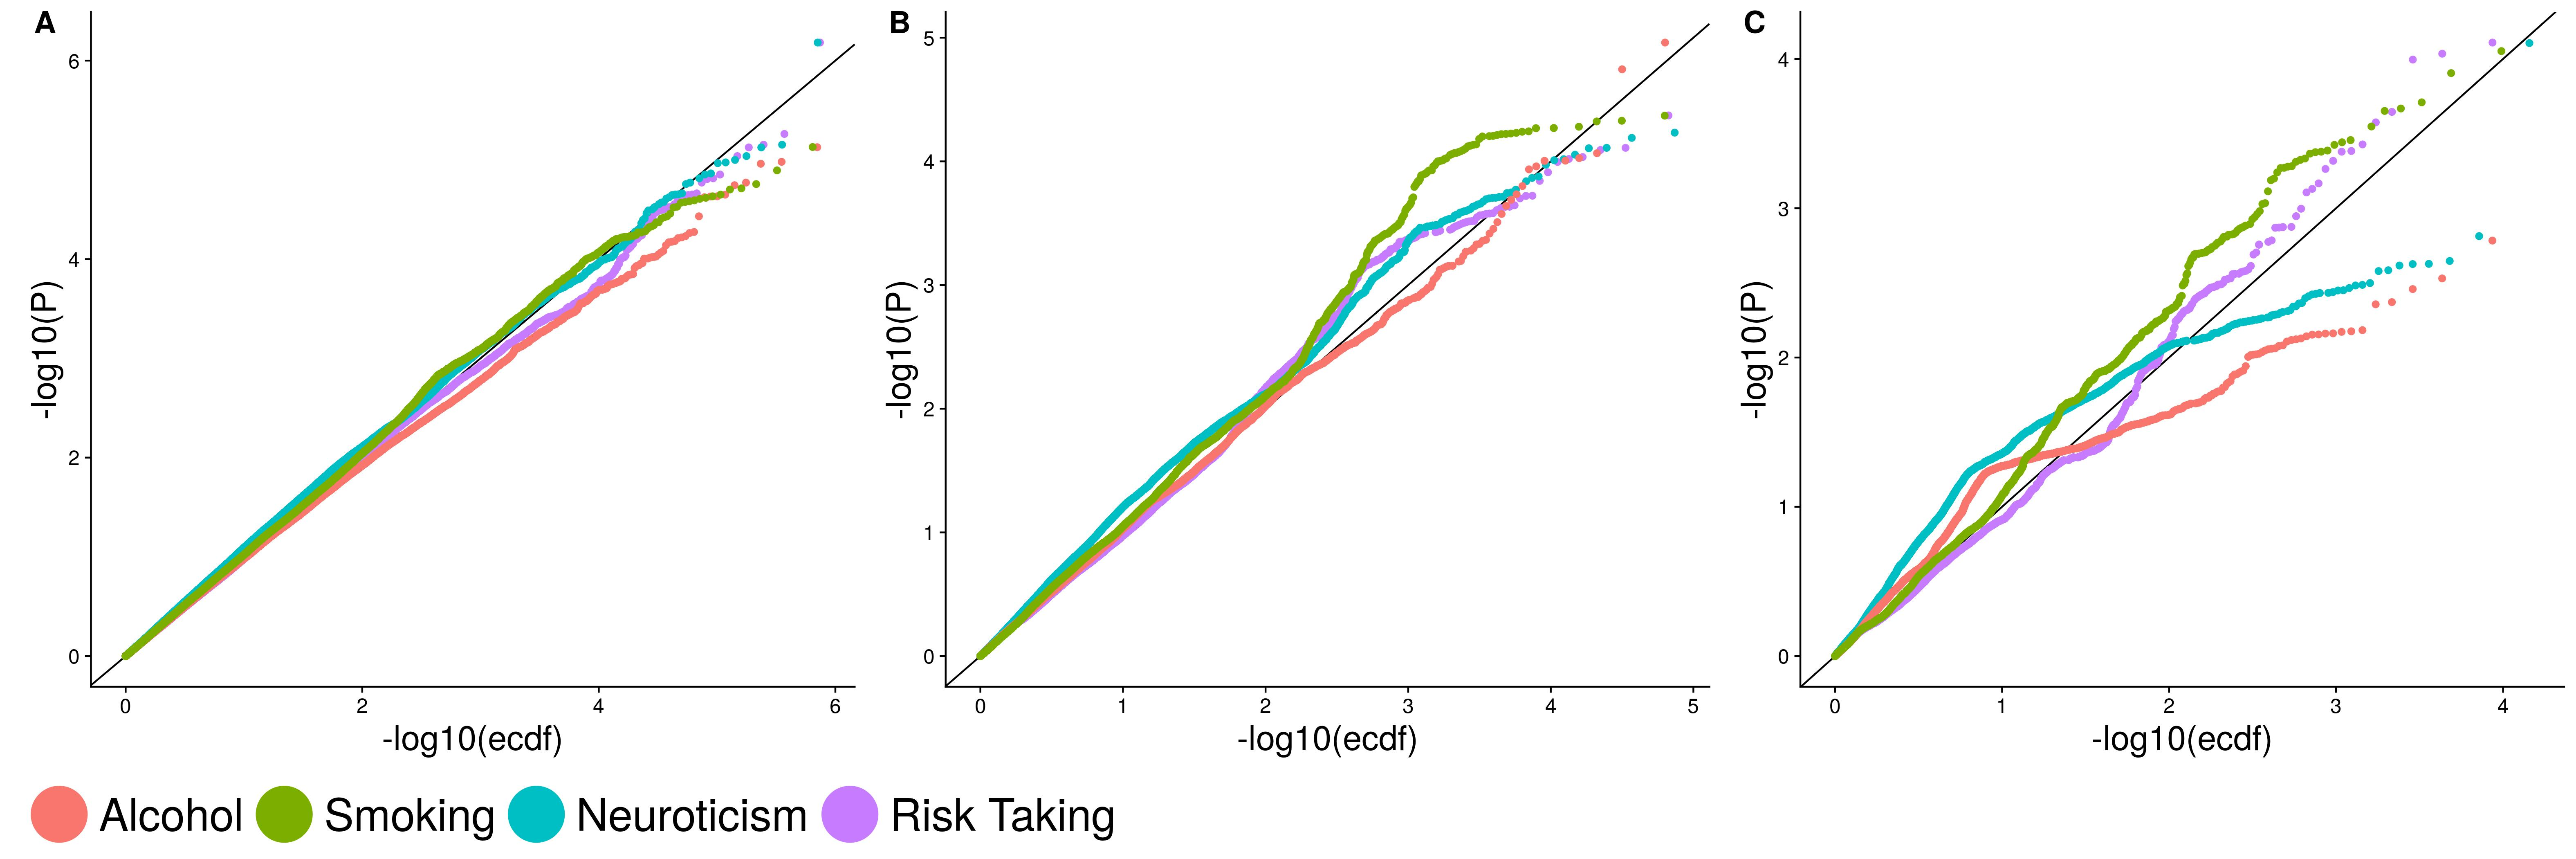
\includegraphics[width=1\linewidth]{ukb_assoc/figure/cFDR/agg_cond.jpeg}
	\end{subfigure}
	\begin{subfigure}{1\textwidth}
		\centering
    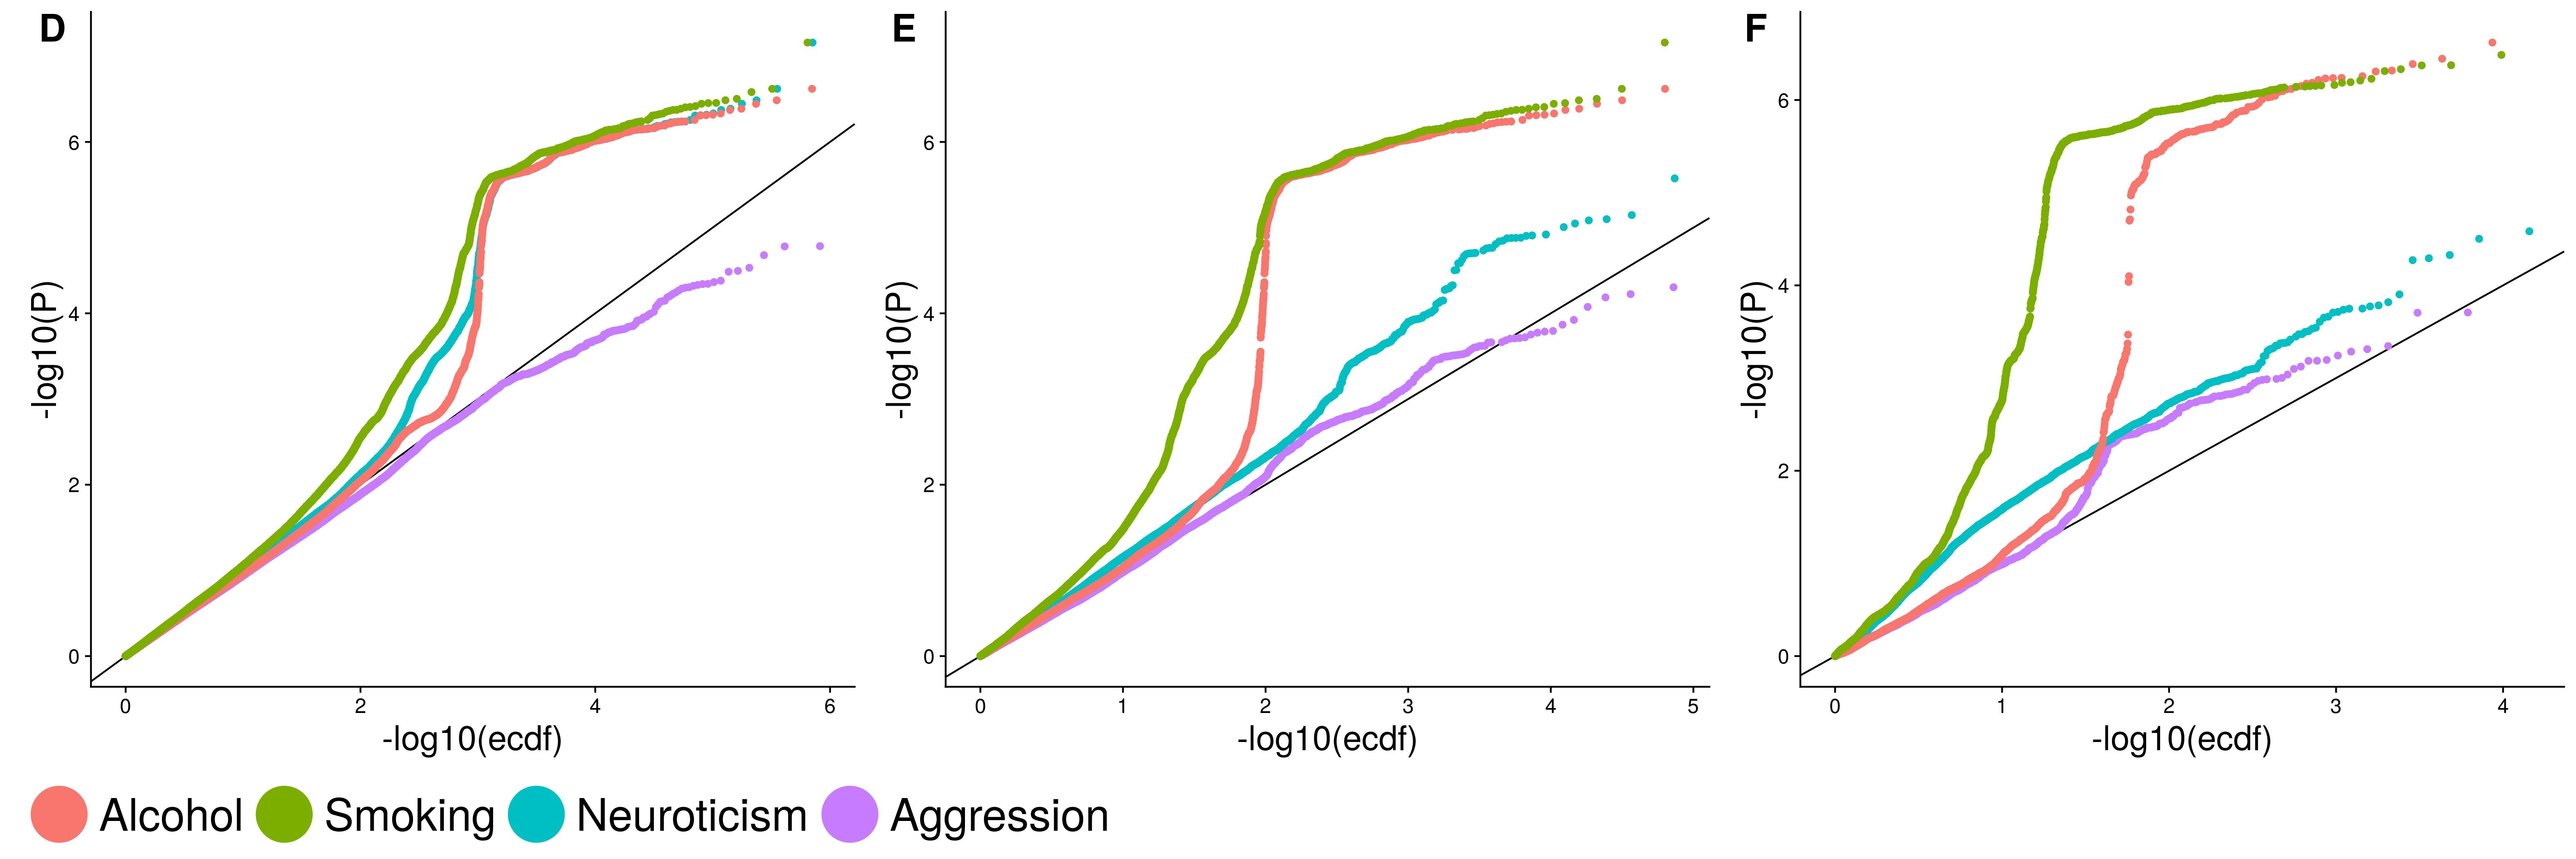
\includegraphics[width=1\linewidth]{ukb_assoc/figure/cFDR/risk_cond.jpeg}
	\end{subfigure}
  \caption{
    Conditional QQ plots for both risk taking and aggression. 
    Figure A-C represents the conditional QQ-plots for impulsive aggression,
    conditional on the remaining phenotypes given threshold $p\leq0.1$, $p\leq0.01$, $p\leq0.001$ respectively.
    Similar, Figure D-F are the conditional QQ-plots for risk taking, conditional on the remaining phenotypes across the three thresholds.\label{fig:cFDR}}
\end{figure}


\begin{table}[htpb]
  %latex.default(dat, title = "", file = "risk_cFDR.tex", cellTexCmds = cell.format,     numeric.dollar = FALSE, digits = 3, rowname = NULL, table.env = F)%
\begin{center}
\begin{tabular}{rlrrlllr}
\hline\hline
\multicolumn{1}{c}{CHR}&\multicolumn{1}{c}{SNP}&\multicolumn{1}{c}{cFDR}&\multicolumn{1}{c}{Z}&\multicolumn{1}{c}{A1}&\multicolumn{1}{c}{A2}&\multicolumn{1}{c}{$\delta$}&\multicolumn{1}{c}{$Z_{\delta}$}\tabularnewline
\hline
    1&   rs1912231&   5.25e-03&    4.34&   C&   T&   Alcohol&    3.62\tabularnewline
    3&   rs9870448&   2.77e-04&   -5.24&   A&   G&   Alcohol&   -3.89\tabularnewline
\bfseries    3&\bfseries   rs570682061&\bfseries   6.64e-05&\bfseries    5.22&\bfseries   A&\bfseries   AT&\bfseries   Smoking&\bfseries    3.67\tabularnewline
    6&   rs7744605&   7.52e-05&    5.16&   C&   A&   Smoking&    3.27\tabularnewline
    6&   rs9468372&   2.06e-04&    4.88&   T&   A&   Smoking&    3.42\tabularnewline
    8&   rs1968400&   9.86e-03&    3.67&   G&   C&   Smoking&    3.23\tabularnewline
    8&   rs116807689&   2.62e-03&    4.16&   A&   G&   Smoking&    3.73\tabularnewline
   10&   rs67657945&   2.13e-03&   -4.23&   CT&   C&   Smoking&   -3.21\tabularnewline
\hline
\end{tabular}\end{center}

  \caption{
    Independent loci ($r^2 < 0.05$) with $cFDR\leq0.01$.
    SNPs are listed by location (CHR) and conditional phenotype ($\delta$).
    Z-scores are indicated for both risk taking and the conditional phenotype.
    Data was adjusted for genomic inflation.
    SNPs in bold indicate replication in an independent sample.
  }\label{tab:cFDR}
\end{table}

\subsection{Genetic Correlations}
\label{sub:genetic_correlations_internal}

Figure~\ref{fig:gcor} displays the genetic correlations of analysed phenotypes.
All correlations were significant after adjusting for multiple testing ($p\leq0.005$).
The largest genetic correlations could be observed between impulsive aggression and neuroticism ($r_g=0.63, SE=0.083, p=4.6496e-14$), 
followed by a considerable correlation between risk taking and aggression ($r_g=0.44, SE=0.1039, p=2.6656e-5$).
Interestingly, relatively large negative correlations are also present between alcohol consumption and aggression ($r_g=-0.39, SE=0.0892, p=1.6942e-5$)
as well as between smoking and aggression ($r_g=0.4, SE=0.0716, p=1.6442e-08$).
Correlation, between smoking and alcohol consumption was not significant as well of neglectable effect ($r_g=0.06, SE=0.044628, p=0.15502$).
Interestingly, these respectively high genetic correlations are not reflected in the corresponding conditional FDR (see Figure~\ref{fig:cFDR}).

Further, risk taking shows non-significant and small correlation with neuroticism ($r_g=-0.12, SE=0.0738, p=0.10629$) and
alcohol consumption ($r_g=0.07, SE=0.051506, p=0.19604$) but the correlation between risk taking and smoking ($r_g=0.34, SE=0.0514, p=2.4044E-11$) is considerable.
In addition, medium correlations were present between neuroticism and alcohol consumption ($r_g=-0.17, SE=0.0406, p=2.6366e-4$). 
Effects were also present between neuroticism and smoking, but did not pass multiple testing ($r_g=0.16, SE=0.0662, p=0.017786$).

\begin{figure}[!h]
	\centering
  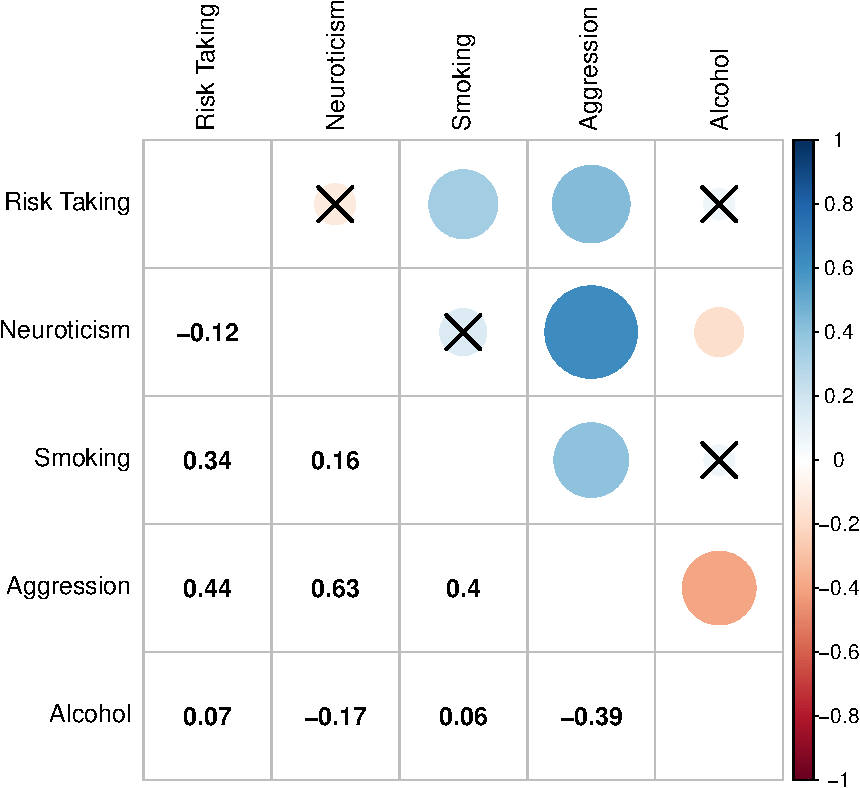
\includegraphics[width=0.8\linewidth]{ukb_assoc/figure/genetic_corr/gcorr_plot_circle_full_se.pdf}
  \caption{Genetic Correlations.
    Pairwise genetic correlations across analysed phenotypes.
    The lower triangular matrix indicate the numeric correlations, while the upper part is a visual representation of the strengths and direction of the correlation.
    A cross indicate a non-significant correlation after adjusting for multiple testing.
  }\label{fig:gcor}
\end{figure}
